\documentclass[12pt]{article}
\usepackage{amsmath}
\usepackage{amsfonts}
\usepackage{amssymb}
\usepackage{graphicx}
\usepackage[left=2cm,right=2cm,top=2cm,bottom=2cm]{geometry}
\author{khanal}


\begin{document}

\hfill \today

\begin{center}
\textbf{\Large MA305 - Classwork \#6\\
	 \large Learn LaTeX by Examples}
\end{center}

\noindent \hrulefill

\noindent \textbf{1. Examples of lists}\\
 
\textit{Unnumbered list.}
\begin{itemize}
\item First item is nothing!
\item Second item is unknown.
\end{itemize}

\vspace{0.25in}

\textit{Numbered list.} 
\begin{enumerate}
\item $\alpha, \beta$, $\alpha$, $\omega$, $\Omega$
\item $f(x)=\dfrac{x^2+4}{x+2}$.
\item Temperature is $75^\circ$ F.
\end{enumerate}

\vspace{0.25in}

\textit{Other styles.}  
\begin{enumerate}
\item[a.] 
\item[b.] 
\end{enumerate}

\begin{itemize}
\item[i.] 
\item[ii.] 
\end{itemize}


\newpage
\noindent \textbf{2. Examples of mathematical expressions} 


$x=2$

\[ x=2\] 

\begin{equation}\label{eq1}
x^2-4=0
\end{equation}

From equation (\ref{eq1}), we get $x=\pm 2$.
%
\[\sin2\theta = 2\sin\theta\cos\theta, \quad \cos2\theta = 2\cos^2\theta -1 =1 -2\sin^2\theta\]
%
$$f(x)=\int_0^x g(t)\, dt \implies f'(x) = g(x)$$

Roots of a quadratic equation $ax^2+bx+c=0$ is given by 
\begin{equation}
x_{1,2}=\frac{-b\pm \sqrt{b^2-4ac}}{2a}
\end{equation} 

\begin{equation*}
\int_0^1 \frac{4}{1+x^2}\, dx = \pi
\end{equation*} 



\begin{eqnarray*}
x_{n+1} &= & x_n-\frac{f(x_n)}{f'(x_n)}\\
x_{n+1} &=& x_n-2\frac{f(x_n)}{f'(x_n)}\\
x_{n+1} &=& x_n-\frac{f(x_n)}{\sqrt{[f'(x_n)]^2-f(x_n)f''(x_n)}}
\end{eqnarray*}

\newpage
\noindent \textbf{3. Examples to create a table} 

\begin{center}
\begin{tabular}{|c|c|c|c|c|c|}
\hline
Food  &  protein & carbohydrate & fat & salt & calcium\\
\hline
	 A	&   0    &     15 	&       10 		&    10 &    15\\
	 B	&  30    &    20   	&     	20   & 10   &  20\\
	 C	&  20    &    25    &    	10   & 20  &   15\\
	 D	&  30    &   15     &  		30    & 10 &    20\\
	 E	&  10    &  15       & 		0    & 20 &     5\\
\hline
\end{tabular}
\end{center}
\vspace{0.1in}

Table in math environment (array). 
\[
\begin{array}{|c|c|c|}
\hline
n & t & y(t)\\
\hline
0 & 0.00 & 0.5000\\
1 & 0.25 & 0.5615\\
2 & 0.50 & 0.6204\\
3 & 0.75 & 0.6752\\
4 & 1.00 & 0.7251\\
\hline
\end{array}
\]

Math expressions with matrix and vectors:
\[
A=
\left[
\begin{array}{rrr}
3&0&1\\
0&3&1\\
1&1&3
\end{array}
\right]
,\quad
A^{-1}= \frac{1}{21}\left[\begin{array}{rrr}
8 & 1 & -3 \\
1 & 8 & -3\\
-3 & -3 & 9
\end{array}\right], \quad
{\bf x}=
\left[
\begin{array}{r}
x_1\\
x_2\\
x_3
\end{array}
\right], \quad
{\bf b}=
\left[
\begin{array}{r}
4\\
4\\
5
\end{array}
\right]
\]

\newpage
\noindent \textbf{4. Example on how to insert a figure in the text}
%%%%%%%%%%%%%%%%%%%%%%%%%%%%%%%%%%%%%%%%%%%%

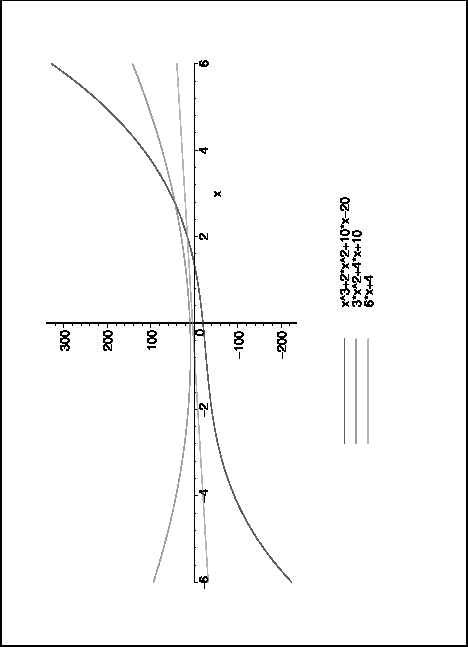
\includegraphics[width=2.in]{plot1.jpg} 

\rotatebox{90}{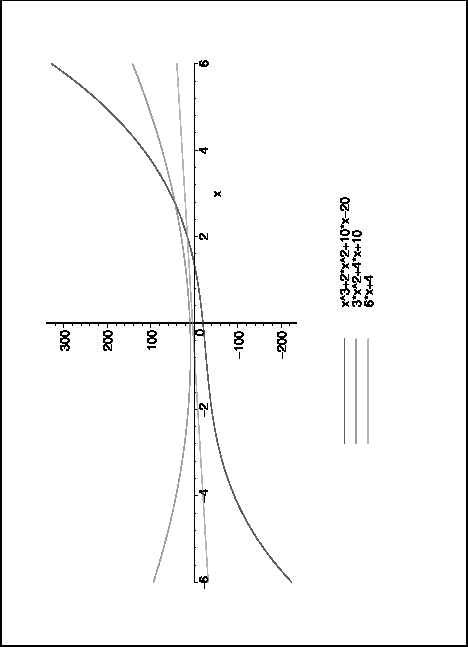
\includegraphics[width=2.in]{plot1.jpg}}


\begin{center}
\rotatebox{270}{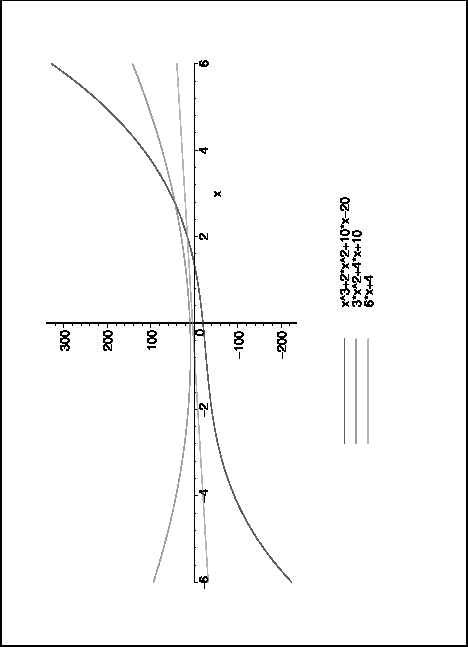
\includegraphics[width=2.5in]{plot1.jpg}}
\end{center}

\newpage
\noindent \textbf{5. Here is an example of how to use verbatim} 

\begin{verbatim}
>> f=inline('x^3+2*x^2+10*x-20');
>> format long
>> xr=fzero(f,[1,2])
   xr=1.368808107821373
\end{verbatim}




\begin{verbatim}
for i=1:10
    f1=x(2)-cos(x(1))^2;
    f2=x(1)^2+x(2)^2-x(1)-2;
    f=[f1; f2];
    J1=[sin(2*x(1)) 1]; %df1/dx, df1/dy
    J2=[2*x(1)-1 2*x(2)]; %df2/dx, df2/dy
    J=[J1; J2]; %Jacobian Matrix
    h=J\f; %h=(J^(-1))f
    x=x-h; %x=x-(J^(-1))f
end
\end{verbatim}

\end{document}
\grid
